\chapter{Graduação}

Na área do Ensino a UFBA oferece cursos de Graduação e Pós Graduação em várias áreas do conhecimento, sob a orientação da Pró-Reitoria de Ensino de Graduação, órgão responsável pelo planejamento, coordenação, acompanhamento e avaliação dos cursos, onde são executadas as diretrizes de funcionamento de acordo com várias resoluções  aprovadas.

\section{Sistemas de Informação}
\index{BSI}
\subsection{Introdução}

O curso de Bacharelado em Sistemas de Informação da UFBA foi criado em 2010. Embora ainda seja uma área recente, já conquistou um espaço relevante no mercado de trabalho. O bacharel em Sistemas de Informação deve planejar e organizar o processamento, o armazenamento e a recuperação de informações, de modo que estas possam ser disponibilizadas aos usuários.

\textcolor{red}{Texto repetido}

O Bacharelado em Sistemas de Informação(SI) foi implantado na Universidade Federal da Bahia(UFBA) no ano de 2010. Apesar de ter menos tempo vigente na Universidade que o curso de Bacharelado em Ciência da Computação (criado em 1968), ambos têm afinidade e andam juntos durante o curso.

O curso alia conhecimentos da computação com gestão em geral, proporcionando ao estudante aprendizados importantes sobre os componentes dos Sistemas de Informação.
  
  \subsection{Coordenação do Colegiado}
       \begin{itemize}
           \item Coordenador: Professor Ricardo Araújo Rios
           \item Vice-Coordenador: Professor Paul Regnier
           \item Sala: 115 do Instituto de Matemática(IM)
           \item Atendimento: Segunda-feira, das 18h às 20h30
           \item Telefone: (71) 3283-6267
           \item E-mail: csi@ufba.br
       \end{itemize}
       
\subsection{Estrutura Curricular}
 \paragraph{Carga Horária}
       O currículo do curso possui uma distribuição de horas-aula seguindo o padrão:
       \begin{itemize}
           \item Eixo Central: 85 por cento, distribuídos por:\\
                Disciplinas obrigatórias: 2346 horas\\
                Atividades complementares: 100 horas\\
                Trabalho de Conclusão do Curso(TCC): 187 horas\\
           \item Componentes curriculares optativos: 15 por cento, distribuídos por:\\
                Disciplinas optativas: 544 horas.\\
            \end{itemize}
        Totalizando a carga horária de 3177 horas.
    
 \paragraph{Componentes Curriculares}
     \begin{itemize}
            \item Eixo Central: As matérias e atividades proporcionadas por esta área fornecem grande formação em Sistema de Informação, Computação e Engenharia de Software. É obrigatório para os alunos a conclusão da carga horária do Eixo, pois as disciplinas são consideradas essenciais e feitas como base para a formação de um bacharel em SI.
            \item Componentes curriculares optativos:
        O currículo permite que o estudante opte por disciplinas que o especializem em sistemas WEB ou e Informática em Saúde.
            \item Disciplinas livres:
        São matérias que têm relação com a Computação ou com formação complementar, que não estão organizadas pelas áreas de concentração.
        \end{itemize}
    
\subsection{Habilidades e Competências}
 \paragraph{Ao concluir o curso de SI, pode-se exercer as seguintes funções:}
       \begin{itemize}
           \item Analista, projetista e programador de sistemas de informação;
           \item Gerente de projetos em informática;
           \item Consultoria em TI e Sistemas de Informação;
           \item Analista de suporte a ambientes computacionais;
           \item Gerente de suporte a ambientes computacionais;
           \item Gerente de divisões organizacionais de tecnologia da informação.
       \end{itemize}
       
\subsection{Pós-formação}
 \paragraph{O que se espera de uma pessoa formada em SI?}
    \begin{itemize}
        \item Solucionar problemas computacionais usando as tecnologias atuais;
        \item Trabalhar em equipe;
        \item  Prestar serviços de Consultoria;
        \item Interagir no meio de forma criativa e modificadora;
        \item Possuam formação complementar em Gestão;
        \item Possam atuar no mercado de trabalho em prestação de serviços de consultoria.
        \end{itemize}

%\textcolor{red}{Utilize o sistema de tabelas adotado pelos alunos que montaram as grades de LCC e BCC}
\newpage
\section{Licenciatura em Computação}

\subsection{Introdução}
O curso de Licenciatura em Computação(LC)\index{LC}, que teve suas atividades iniciadas em 2010, é oferecido pelo Instituto de Matemática e Estatística(IME) e segue as Diretrizes Curriculares Nacionais para a formação de professores da Educação Básica em Nível Superior, além de acompanhar as constantes transformações nos âmbitos científicos, educacionais e tecnológicos. 

A proposta do curso foi elaborada pela comissão escolhida pelo Departamento de Ciência da Computação, composta pelas professoras Anna Friedericka Schwarzelmüller, Débora Abdalla Santos e Laís Nascimento Salvador. As professoras contaram com a colaboração dos professores Aline Maria Santos Andrade, Celso Alberto Saibel Santos, Daniela Barreiro Claro e Manoel Gomes de Mendonça Neto, para suporte nas disciplinas com conteúdos da área tecnológica principalmente.

\subsection{Colegiado do Curso}
\begin{itemize}
	\item {Coordenadora: Anna Friedericka Schwarzelmuller}
    \item {Vice-coordenador: Ecivaldo Matos}
    \item {Sala do colegiado: 116 do Instituto de Matemática}
    \item {E-mail para contato: lc@ufba.br}
\end{itemize}

\subsection{Objetivos do Curso}
%\paragraph{} %Nao utilizar esse comando
    O site do curso de LC da UFBA define:
        \begin{quote}
        {\small De maneira geral pode-se estabelecer como objetivo do curso, formar profissionais de educação que atuem como agentes integradores no processo de ensino-aprendizagem, capazes de compreender o fenômeno educativo na sua diversidade e complexidade, contextualizando-o socialmente no seu tempo e    espaço.}
        \end{quote}

Vale acrescentar diversos outros objetivos. Primeiramente têm-se a finalidade de fornecer uma formação bem estruturada e sólida na compreensão dos problemas que envolvem a área de Ensino e inserção da tecnologia nesse meio.

Também, em uma área em constante mudança e aprimoramento, o curso traz uma proposta de gerar inovações durante a formação dos futuros educadores. Esses poderão exercer o magistério e estarão preparados para o mercado de trabalho.

Por fim, propõem-se a incentivar o aluno a programas de pós-graduação e o seu espírito científico.

\subsection{Perfil do Egresso}

O formando sai do curso preparado para atuar no magistério em nível de ensino básico, técnico e tecnológico, tendo qualificações pedagógicas e científicas. Espera-se que o egresso tenha domínio em aspectos básicos de ciência da computação e na área de educação, sendo capaz de realizar projetos interdisciplinares com outros docentes, e utilizar de tecnologias digitais para mudar positivamente o processo de aprendizado do estudante. 

Além disso, terá formação para ingressar em pós-graduação e em programas de ciência da computação ou outras áreas do gênero.

\subsection{Campos de Atuação}

O profissional formado em LC pode atuar como docente em ensino fundamental, médio e escolas técnicas, trabalhar com treinamento e qualificação em corporações, como consultor em empresas e instituições, e consultor técnico. Outras opções são empreendedorismo, avaliando e desenvolvendo softwares educacionais e de atividades de pesquisa na área de informática.

\subsection{Dados Gerais do Curso}
    \paragraph{Tempo de duração}
    \begin{quote}
	    \begin{itemize}
		    \item{Duração Mínima: 3.5 anos}
            \item{Duração Máxima: 7.5 anos}
	    \end{itemize}  
    \end{quote}

    \paragraph{Carga Horária}
    \begin{quote}
	    \begin{itemize}
    	    \item{Carga Horária Obrigatória: 2499 horas}
            \item{Carga Horária Optativa: 442 horas}
            \item{Atividade Complementar: 200 horas}
        \end{itemize}
    \end{quote}

\subsection{Base Curricular}
    \paragraph{}A grade curricular de LC possui foco em matérias de computação, matemática e especialmente pedagogia, que são um grande diferencial quando se compara esse curso com o curso de Bacharelado em Ciência da Computação e Sistema de Informação. Matérias como Filosofia da Educação e Fundamentos Psicológicos da Educação são exemplos que formam a base para profissionais da área de pedagogia. 


\begin{longtable}{K{1.7cm}K{6cm}K{1.4cm}K{0.9cm}K{1.5cm}}
\hline
\multicolumn{5}{c}{\textbf{Licenciatura em Computação}}\\
\hline
\multicolumn{5}{c}{\textbf{1$^o$ período}}\\
\hline
 Código & Nome da disciplina & (T-P-E) & C.H. & Requisitos\\
 \hline
EDCB80 & Filosofia da Educação & (2-2-0) & 68 & \\
MATA01 & Cálculo A & (4-0-0) & 68 \\
MATA37 & Introdução à Lógica de Programação & (2-2-0) & 68 & \\
MATA39 & Seminários de Introdução ao Curso & (3-0-0) & 51 \\
MATA42 & Matemática Discreta I & (4-0-0) & 68 \\
 \hline
\multicolumn{2}{c}{TOTAL} & 19 & 323\\
 \hline
 \multicolumn{2}{c}{TOTAL ACUMULADO} & 19 & 323\\
 
 \multicolumn{5}{c}{\textbf{2$^o$ período}}\\
\hline
 Código & Nome da disciplina & (T-P-E) & C.H. & Requisitos\\
 \hline
EDC287 & Educação e Tecnologias Contemporâneas & (2-2-0) & 68\\
MATD04 & Estrutura de Dados & (2-2-0) & 68 & MATA37\\
MATC81 & Sistemas Básicos de Computação:
Arquitetura e Software & (2-2-0) & 68 & MATA39\\
MATA97 & Introdução à Lógica Matemática & (2-2-0) & 68 & MATA42\\
MATA68 & Computador, Ética e Sociedade & (2-1-0) & 51\\
 \hline
\multicolumn{2}{c}{TOTAL} & 19 & 323\\
 \hline
 \multicolumn{2}{c}{TOTAL ACUMULADO} & 38 & 646\\
 \hline
 
 \multicolumn{5}{c}{\textbf{3$^o$ período}}\\
\hline
 Código & Nome da disciplina & (T-P-E) & C.H. & Requisitos\\
 \hline
EDCA01 & Fundamentos Psicológicos da Educação & (2-2-0) & 68 & \\
MATA55 & Programação Orientada a Objetos  & (2-2-0) & 68 & MATD01 \\
MAT236 & Métodos Estatísticos & (4-0-0) & 68 & MATA01 MATA42 \\
MATC74 & Introdução a Linguagens Formais e Autômatos & (2-2-0) & 68 & MATA42\\
OPT01 & --- & --- & 51 \\
 \hline
\multicolumn{2}{c}{TOTAL} & 19 & 323\\
 \hline
 \multicolumn{2}{c}{TOTAL ACUMULADO} & 57 & 969\\
 \hline
 
 \multicolumn{5}{c}{\textbf{4$^o$ período}}\\
\hline
 Código & Nome da disciplina & (T-P-E) & C.H. & Requisitos\\
 \hline
EDCA11 & Didática e Práxis Pedagógica I & (0-4-0) & 68 & \\
MATA62 & Engenharia de Software I & (2-2-0) & 68 & MATA55 \\
MATC82 & Sistemas Web & (2-2-0) & 68 & MATA55\\
MATA59 & Redes de Computadores I & (2-2-0) & 68 & MATC81\\
MATA41 & Informática na Educação & (2-2-0) & 68 \\
 \hline
\multicolumn{2}{c}{TOTAL} & 20 & 340\\
 \hline
 \multicolumn{2}{c}{TOTAL ACUMULADO} & 77 & 1309\\
 \hline
 
 \multicolumn{5}{c}{\textbf{5$^o$ período}}\\
\hline
 Código & Nome da disciplina & (T-P-E) & C.H. & Requisitos\\
 \hline
EDCA12 & Didáticas e Práxis Pedagógicas II & (0-4-0) & 68 & EDCA11 \\
MATB19 & Sistemas Multimídias  & (2-2-0) & 68 & MATA55 \\
MATD05 & Banco de Dados e Aplicações & (2-2-0) & 68 & MATD04 \\
MATB21 & Ambientes Interativos de Aprendizagem & (4-0-0) & 68 & MATA37 MATA41\\
EDC286 & Avaliação de Aprendizagem & (2-2-0) & 68 \\
 \hline
\multicolumn{2}{c}{TOTAL} & 20 & 340\\
 \hline
 \multicolumn{2}{c}{TOTAL ACUMULADO} & 97 & 1649\\
 \hline
 \newpage
 \hline
 
  \multicolumn{5}{c}{\textbf{6$^o$ período}}\\
\hline
 Código & Nome da disciplina & (T-P-E) & C.H. & Requisitos\\
 \hline
MATC68 & Estágio Supervisionado I & (0-0-4) & 68 & EDCA11 EDCA12\\
MATC72 & Interação Humano-Computador & (2-2-0) & 68 & MATB19 \\
MATC78 & Projeto de Software Educativo & (2-2-0 & 68 & MATA62\\
MATB22 & Laboratório de Informática na Educação & (0-3-0) & 51 & MATB21\\
MATC76 & Prática de Ensino de Computação I & (0-4-0) & 68 & EDCA11\\
 \hline
\multicolumn{2}{c}{TOTAL} & 19 & 323\\
 \hline
 \multicolumn{2}{c}{TOTAL ACUMULADO} & 116 & 1972 \\
 \hline
 
  \multicolumn{5}{c}{\textbf{7$^o$ período}}\\
\hline
 Código & Nome da disciplina & (T-P-E) & C.H. & Requisitos\\
 \hline
MATC69 & Estágio Supervisionado II & (0-0-4) & 68 & MATC68\\
MATC79 & Projetos Interdisciplinares: concepçao e ética  & (1-3-0) & 68 & EDCA11 MATA41 \\
MATB20 & Inteligência Artificial em Educação & (2-2-0) & 68 & MATA41, MATC73 \\
MATC77 & Prática de Ensino de Computação & (0-4-0) & 68 & MATA41 MATC73\\
OPT02 & --- & --- & 51 \\
 \hline
\multicolumn{2}{c}{TOTAL} & 19 & 323\\
 \hline
 \multicolumn{2}{c}{TOTAL ACUMULADO} & 135 & 2295\\
 \hline
 
   \multicolumn{5}{c}{\textbf{8$^o$ período}}\\
\hline
 Código & Nome da disciplina & (T-P-E) & C.H. & Requisitos\\
 \hline
MATC70 & Estágio Supervisionado III & (0-0-6) & 102 & MATC69\\
LETE46 & Libras-Língua Brasileira de Sinais & (1-1-0) & 34\\
OPT03 & --- & --- & 68\\
OPT04 & --- & --- & 51\\
OPT05 & --- & --- & 51\\
 \hline
\multicolumn{2}{c}{TOTAL} & 18 & 306\\
 \hline
 \multicolumn{2}{c}{TOTAL ACUMULADO} & 153 & 2601\\
 \hline
 
 
   \multicolumn{5}{c}{\textbf{9$^o$ período}}\\
\hline
 Código & Nome da disciplina & (T-P-E) & C.H. & Requisitos\\
 \hline
MATC69 & Estágio Supervisionado IV & (0-0-10) & 170 & MATC70\\
OPT06 & --- & --- & 68 \\
OPT07 & --- & --- & 51 \\
OPT08 & --- & --- & 51 \\
 \hline
\multicolumn{2}{c}{TOTAL} & 20 & 340\\
 \hline
 \multicolumn{2}{c}{TOTAL ACUMULADO} & 173 & 2941\\
 \hline
\end{longtable}

Legenda:\\
{\bf C.H.} Carga Horária\\
{\bf T} Carga horária de aula teórica\\
{\bf P} Carga horária de aula prática\\
{\bf E} Carga horária de estágio\\


\newpage
\section{Bacharelado em Ciência da Computação} \index{BCC}

	\subsection{Introdução}
	O curso de Computação da UFBA foi o primeiro curso de graduação no Brasil nesta área ao lado do curso de Ciência da Computação da UNICAMP. Começou com o nome de Bacharelado em Processamento de Dados e inciou suas atividades em 03/03/1969 e alia o estudo da arte da ciência e da tecnologia da computação.

	\subsection{Coordenação do Colegiado}
    \begin{itemize}
        \item  Coordenador: Luciano Rebouças de Oliveira
        \item  Vice-Coordenador: Rubisley Lemes
        \item  Sala: 116 do Instituto de Matemática e Estatística(IME)
        \item  Atendimento: Terças e Quintas 14h às 16h
        \item Telefone: (71) 3283-6271
        \item E-mail: ccc@ufba.br
    \end{itemize}
    
    \subsection{Objetivos}
    O objetivo do curso é fornecer conhecimento e práticas para que o egresso esteja situado no campo da tecnologia e da computação. Ele, em sua finalidade, irá nos fornecer uma formação básica porém sólida da teoria da computação, apresentando conceitos da computação e de áreas da tecnologia que utilizem da computação. Também faz parte do objetivo do curso dar uma formação que torne o egresso, um pesquisador da área da computação ou de áreas afins, e capacitá-lo, para que esteja pronto para o mercado de trabalho, tanto no campo industrial, quanto no acadêmico; e a capacidade necessária para ingressar em programas de pós-graduação na área da computação ou áreas afins.
    
    \subsection{Perfil do Egresso}
    O Perfil do Egresso entende-se como as habilidades e competências que o egresso deverá possuir ao concluir o curso. Os egressos do curso devem estar preparados para atuar no mercado de trabalho propondo soluções adequadas que utilizem o computador bem como ter maturidade e conhecimento para atuar de maneira inovadora, contribuindo com o desenvolvimento tecnológico da área da Computação. Eles devem ter uma base científica que os tornem aptos a se tornarem futuros pesquisadores; tenha a capacidade de atuar de maneira multidisciplinar, aplicando a computação em varias áreas de conhecimento. Faz parte do perfil do egresso do curso, atuar como um engenheiro de software, e ter os fundamentos para trabalhar em equipe, principalmente no projeto de sistemas de sistemas.
    
    
    
    \subsection{Distribuição da Carga Horária}
    Algumas normas devem ser definidos pelo Colegiado do Curso. Para o aluno receber o diploma de Bacharel em Ciência da Computação ele deve cursar ma carga horária total de no mínimo de 3.347 horas distribuídas em média em 8 semestres, cumprindo com os seguintes requisitos; 
    \begin{itemize}
        \item  Cursar as disciplinas obrigatórias do curso que totalizam 2.346 horas; 
        \item  Cursar as disciplinas optativas do curso que totalizam 714 horas; 
        \item  Realizar trabalho de conclusão de curso sob a orientação de um professor com apresentação e defesa de uma monografia, com 187 horas de carga horária dividida em 2 componentes curriculares obrigatórios; 
        \item  Cumprir 100 horas de atividades complementares.
    \end{itemize}



\subsection{Elenco de componentes curriculares}
Os componentes curriculares são divididos quanto à natureza em obrigatórios e optativos, e quanto à modalidade em disciplinas, atividades complementares e trabalho de conclusão de curso.
\subsubsection{Pré-requisitos}
 As disciplinas estão relacionadas entre si no que é chamado de pré-requisito, que pode ser obrigatório ou não. Se uma disciplina A é pré-requisito obrigatório de B, você só pode cursar a disciplina B se já tiver sido aprovado na disciplina A. Se uma disciplina A é pré-requisito recomendado de B, recomenda-se que você curse a disciplina A anteriormente ou paralelamente à disciplina B. A disciplina A é pré-requisito recomendado de B quando: 
\begin{itemize}
    \item Noções de conteúdos da disciplina A são utilizados em B, mas o aluno pode obter essas noções sozinho, sem cursar a disciplina A;
    \item Os estudos da disciplina A podem facilitar o aprendizado da disciplina B, assim como podem auxiliar o aluno a propor soluções mais elaboradas para alguns problemas apresentados na disciplina B e até tornar o estudo dos conteúdos de B mais aprofundados;
    \item Conteúdos do ensino médio importantes para o aprendizado dos conteúdos da disciplina B são revisados na disciplina A. 
\end{itemize}
\subsubsection{Componentes curriculares optativos}
O aluno pode cursar os componentes curriculares optativos através de áreas de concentração, perfis complementares ou escolher uma formação genérica. No caso das áreas de concentração, você se direciona a uma área específica da Ciência da Computação, já os perfis complementares direcionam o aluno a disciplinas que façam uma relação da Informática com outras áreas. Caso você não queira escolher nenhuma dessas duas direções, é possível escolher uma formação genérica, na qual o aluno cursa disciplinas optativas mais variadas.

Você pode encontrar exemplos de áreas de concentração e perfis complementares com suas disciplinas no Projeto Pedagógico para o curso de Bacharelado em Ciência da Computação, das páginas 9 à 15, disponível em

https://wiki.dcc.ufba.br/pub/CCC/EstruturadoCurso/reforma2011.pdf
\subsubsection{Componentes curriculares obrigatórios}
 A figura abaixo é um fluxograma que apresenta o andamento do curso em sua situação ideal, com as disciplinas obrigatórias indicadas por código, nome e carga horária. A setas indicam que uma matéria é pré-requisito obrigatório da outra. Por isso, as disciplinas estão divididas por semestre de forma que fiquem ordenadas obedecendo os pré-requisitos e a carga horária semestral fique equilibrada.

As disciplinas optativas estão divididas em 6 de 68 horas e 6 de 51 horas, mas essa divisão não é obrigatória. Desde que curse pelo menos as 714 horas de matérias optativas, a quantidade de disciplinas e a forma em que essas horas estão divididas é de livre escolha do aluno.

Currículo acadêmico do curso de Bacharelado em Ciência da Computação, aprovado em 09/2011, válido para todos os alunos ingressos a partir de 2012.1.

%\begin{table}[h]
%\centering
\begin{longtable}{K{1.7cm}K{6cm}K{1cm}K{0.9cm}K{1.5cm}}
\toprule
\multicolumn{5}{c}{\textbf{Bacharelado em Ciência da Computação}}\\
\midrule
\multicolumn{5}{c}{\textbf{1$^o$ período}}\\
\midrule
 Código & Nome da disciplina & (T-P) & C.H. & Requisitos\\
\midrule
MATA01 & Geometria Analítica & (4-0) & 68 & \\
MATA02 & Cálculo A & (6-0) & 102 \\
MATA37 & Introdução à Lógica de Programação & (2-2) & 68 & \\
MATA38 & Projeto de Circuitos Lógicos & (4-0) & 68 \\
MATA39 & Seminários em Computação & (3-0) & 51 \\
MATA42 & Matemática Discreta I & (4-0) & 68 \\
 \midrule
\multicolumn{2}{c}{TOTAL} & 25 & 425\\
 \midrule
 \multicolumn{2}{c}{TOTAL ACUMULADO} & 23 & 425\\
 \midrule
 \multicolumn{5}{c}{\textbf{2$^o$ período}}\\
\midrule
 Código & Nome da disciplina & (T-P) & C.H. & Requisitos\\
 \midrule
MATA48 & Arquitetura de Computadores a & (4-0) & 68 & MATA38 \\
MATA40 & Estrutura de Dados e Algoritmos I & (2-2) & 68 & MATA37\\
MATA57 & Laboratório de Programação I & (0-3) & 51 & MATA37\\
MATA97 & Matemática Discreta II & (4-0) & 68 & MATA42\\
MATA95 & Complementos de Cálculo & (6-0) & 102 & MATA01 e MATA02\\
MATA07 & Álgebra Linear A & (4-0) & 68 & MATA01\\

 \midrule
\multicolumn{2}{c}{TOTAL} & 25 & 425\\
 \midrule
 \multicolumn{2}{c}{TOTAL ACUMULADO} & 50 & 850\\
 \midrule
 
 \multicolumn{5}{c}{\textbf{3$^o$ período}}\\
\midrule
 Código & Nome da disciplina & (T-P) & C.H. & Requisitos\\
 \midrule
MATA55 & Programação Orientada a Objetos & () & 68 & MATA40 \\
MATA49 & Programação de Software Básico & () & 68 & MATA48, MATA40 e MATA57\\
MATA50 & Linguagens Formais e Autômatos & () & 68 & MATA42\\
MATA47 & Lógica para Computação  & () & 68 & MATA97\\
MAT236 & Métodos Estatísticos  & () & 68 & MATA95\\
FISA75 & Elementos de Eletromagnetismo e Circuitos Elétricos & () & 102 & MATA95\\

 \midrule
\multicolumn{2}{c}{TOTAL} &  & \\
 \midrule
 \multicolumn{2}{c}{TOTAL ACUMULADO} &  & \\
 \midrule
 
\end{longtable}

\noindent
Legenda
%\vspace{0.1cm}
\begin{small}
\begin{description}
\item[C.H.] Carga horária
\item[T] Carga horária de aula teórica
\item[P] Carga horária de aula prática
\end{description}
\end{small}



\chapter{Pós-Graduação}
\section{Programa de Pós-Graduação em Ciência da Computação}

O Programa de Pós-Graduação em Ciência da Computação (PGCOMP) da Universidade Federal da Bahia (UFBA), aprovado pela CAPES, oferece os cursos de Mestrado em Ciência da Computação e de Doutorado em Ciência da Computação, com o objetivo de dar suporte à formação de pesquisadores com competência para gerar novos conhecimentos, conduzir projetos de investigação científica e exercer atividades de docência no Ensino Superior (graduação e pós-graduação lato sensu e stricto sensu) nas áreas de Ciência da Computação e Tecnologia da Informação e Comunicação (TIC).

\subsection{Grupos de Pesquisa}

A maior parte da pesquisa realizada no DCC está ligada aos cursos de pós-graduação apoiados e ao 
    seu corpo docente, atuante em diversas áreas, linhas, grupos de pesquisa, que dentre outros são os seguintes:

\subsubsection{Laboratorio de Sistemas Distribuídos} 
\begin{wrapfigure}{R}{0.3\textwidth}
            \centering
            
\includegraphics[scale = 0.4]{logolasid.png}
        \end{wrapfigure}  
O Laboratório de Sistemas Distribuídos ( LaSiD) é um laboratório de pesquisa dentro do Departamento de Ciência da Computação na Universidade Federal da Bahia (UFBA) . Trata-se de membros do corpo docente do Departamento de Ciência da Computação , assistentes de pesquisa e estudantes de pesquisa ( Ph.D, MSc. E Licenciatura). A missão da LaSiD é desenvolver métodos, técnicas e ferramentas que ajudam na concepção de sistemas distribuídos corretas e confiáveis, a preparar a próxima geração de pesquisadores e desenvolvedores nestas áreas por investigar problemas desafiadores.
\newline
\newline
\newline
\newline\subsubsection{Laboratório de Engenharia de Software}
\begin{wrapfigure}{R}{0.3\textwidth}
            \centering
            
\includegraphics[scale = 0.4]{les.jpg}
        \end{wrapfigure}

O objetivo do Laboratório de Engenharia de Software da Universidade Federal da Bahia ( LES- UFBA) é estudar a disciplina de engenharia de software , bem como áreas que impactam a maneira como se desenvolve, mantém e gerencia software. LES tem vários grupos de pesquisa que investigam diferentes sub-áreas de engenharia de software.


\subsubsection{Web and Interactive Systems Research Group}
\begin{wrapfigure}{R}{0.3\textwidth}
            \centering
            
\includegraphics[scale = 0.2]{logoWISER.png}
        \end{wrapfigure}
O grupo realiza pesquisas nas áreas de Internet e Web voltadas para Web Semântica, Sistemas de Recomendação para Web, Serviços Web, Computação em Nuvem, Web e Internet das Coisas, Internet do Futuro, Recuperação da Informação na Web, Sistemas Interativos, Cidades Inteligentes e Tecnologias Assistivas. O grupo participou e participa de projetos em colaboração com outras instituições nacionais e internacionais.

\subsubsection{Inteligent Vision Research Lab}
\begin{wrapfigure}{R}{0.3\textwidth}
            \centering
            
\includegraphics[scale = 0.4]{logo_ivision.png}
        \end{wrapfigure}
As principais áreas de investigação Vision Lab estão em sistemas interactivos , detecção de objetos , imagem desempenho da classificação , compreensão cena em imagens , avaliação de classificadores de imagens , reconhecimento de ação , entre outros performance. Todas as pesquisas abrangem os campos de Cidades Inteligentes , Sistemas Inteligentes de Transporte e Sistemas biométricos.
	  
	  Um importante objetivo do laboratório é fornecer aplicações do mundo real; para isso, arquiteturas paralelas também estão sendo investigados , a fim de acelerar os sistemas propostos . Sob essa perspectiva , nós dirigimos a nossa pesquisa de requisitos acadêmicos para as necessidades da indústria , da visão a relação integrativa entre estes dois mundos.


\subsubsection{Software Desing and Evolution Group}
\begin{wrapfigure}{R}{0.3\textwidth}
            \centering
            
\includegraphics[scale = 0.4]{desig.jpg}
        \end{wrapfigure}
O design de software requer esforço e inteligência de pessoas para a criação de artefatos de software idealmente concebidos para realizar funções úteis para pessoas. E software útil está em constante evolução. Nesse contexto, o grupo de pesquisa aSide @UFBA tem como objetivo investigar aspectos da ``ciência do artificial'' e de seus processos de design e evolução de software, buscando caracterizar, desenvolver e avaliar modelos, princípios, práticas e ferramentas para que pessoas possam criar, desenhar, construir, validar, reutilizar, modificar, analisar, gerenciar e desfrutar de software de qualidade. 
	  
	  O aSide @ UFBA é um grupo de pesquisa certificado pela UFBA no Diretório de Grupos do CNPq e está associado ao Laboratório de Engenharia de Software (LES) da UFBA.


\subsubsection{Context and Ubiquitous Systems Group CEManTIKA}
\begin{wrapfigure}{R}{0.3\textwidth}
            \centering
            
\includegraphics[scale = 0.8]{cemantica.jpg}
        \end{wrapfigure}
O Grupo CEManTIKA visa estudar conceitos, técnicas, modelos e ferramentas que apoiem a construção de sistemas sensíveis ao contexto. São objetivos do grupo: 

\begin{itemize}
\item Desenvolver sistemas sensíveis ao contexto voltados para diferentes áreas; 
\item  Formalizar conceitos e metamodelos para modelagem de informações de contexto; 
\item  Investigar algoritmos e técnicas de apoio ao processamento do contexto usando raciocínio lógico; 
\item Desenvolver ferramentas de apoio ao projeto e implementação de sistemas sensíveis ao contexto. 
\end{itemize}

\subsubsection{Formalisms and Semantic Applications Research Group}
\begin{wrapfigure}{R}{0.3\textwidth}
            \centering
            
\includegraphics[scale = 0.4]{formas.jpg}
        \end{wrapfigure}
Objetivo principal é estudar , analisar e avaliar abordagens semânticas , cobrindo desde formalismos através de aplicações . As nossas principais áreas de investigação do grupo baseiam-se em cinco etapas principais em conseguir semântica: Métodos , ontologia, Extração de Informação , a interoperabilidade e validação formal . Lamentamos profundamente analisar cada uma dessas abordagens com foco na obtenção de altos níveis de compreensão semântica e pragmática.


\subsubsection{Grupo de Algoritmos e Computação Distribuida Gaudi}
\begin{wrapfigure}{R}{0.3\textwidth}
            \centering
            
\includegraphics[scale = 0.4]{gaudi.jpg}
        \end{wrapfigure}

O GAUDI visa o entendimento dos problemas fundamentais que surgem na confecção de sistemas e aplicações computacionais e a busca de soluções para os mesmos. A sua principal linha de pesquisa concentra-se no estudo de algoritmos distribuídos e na sua aplicação para o desenvolvimento de componentes de software que facilitem a construção de sistemas confiáveis. 

Linhas de Pesquisa: Algoritmos Distribuídos, Tolerância a Falhas, Componentes Distribuídos, Grades Computacionais, Redes Móveis Ad-Hoc (Manets), Teoria dos Grafos.

\subsubsection{Formal Meethods in Software Engineering Group}
\begin{wrapfigure}{R}{0.3\textwidth}
            \centering
            
\includegraphics[scale = 0.4]{MEFES.jpg}
        \end{wrapfigure}
Visa a proposição de processos de desenvolvimento de softwares que sejam sistemáticos, baseados em métodos e ferramentas, e aplicáveis a sistemas reais. Tendo sempre em mente a produção de software de qualidade, dentro de limites previsíveis de tempo e custo.

\subsubsection{Reuse in Software Engineering Group RiSE}
\begin{wrapfigure}{R}{0.3\textwidth}
            \centering
            
\includegraphics[scale = 0.4]{RISE.png}
        \end{wrapfigure}
O objetivo deste projeto é investigar e definir um processo para o desenvolvimento de linhas de produtos orientadas a serviços . O processo proposto envolve as fases de definição de escopo , requisitos e design. Definir um programa de reutilização de software para educar engenheiros de software high- especializados centrados em princípios de reutilização e ideias.

\subsubsection{Software Visualization Group SoftVis}
\begin{wrapfigure}{R}{0.3\textwidth}
            \centering
            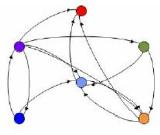
\includegraphics[scale = 0.4]{logoSoftVis.jpg}
        \end{wrapfigure}
O grupo tem como objetivo desenvolver metodologias , ferramentas e técnicas para visualização de software ( SoftVis ) e empiricamente caracterizar e avaliá-los. Tem o interesse especial no desenvolvimento de ambientes SoftVis que podem ser integrados para IDEs para reforçar atividades de compreensão de software e ajudar em tarefas de engenharia de software . Com esse objetivo , temos desenvolvido vários projetos.

\subsubsection{Sistemas de Tempo Real}
\begin{wrapfigure}{R}{0.3\textwidth}
            \centering
            
\includegraphics[scale = 0.4]{sterlogo.png}
        \end{wrapfigure}
Grupo de pesquisa focada no desenvolvimento de novas técnicas para a concepção, análise e implementação de sistemas de tempo real. O nosso grupo foi oficialmente certificada pela UFBA em maio de 2014. A nossa equipa tem vindo a investigar vários aspectos dos sistemas em tempo real , com especial ênfase no multiprocessador / multicore escalonamento de tempo real.

\subsubsection{ONDA DIGITAL - Grupo de Pesquisa e Extensão em Informática, Educação e Sociedade}
\begin{wrapfigure}{R}{0.3\textwidth}
            \centering
            
\includegraphics[scale = 0.2]{logoGPOndaDigital.png}
        \end{wrapfigure}
Grupo de Pesquisa e Extensão em Informática, Educação e Sociedade tem como eixo integrador as relações interdisciplinares entre Computação, Educação e Sociedade com especial interesse nas seguintes áreas: 
\begin{enumerate}
\item informática na educação; 
\item  interação humano-computador (teoria, desenvolvimento e avaliação de tecnologias interativas); 
\item educação em computação; 
\item informática, educação e sociedade.
\end{enumerate}

Desde 2004 o grupo tem estabelecido parcerias com a indústria de software, instituições educacionais e outros parceiros financiadores de projetos. Mais de 100 estudantes de graduação passaram pelo grupo ao longo dos últimos dez anos. Atualmente temos mais de 40 alunos, entre pesquisadores, estudantes de graduação, mestrado e doutorado.

\subsubsection{Computational Intelligence and Optimization Research Lab}
\begin{wrapfigure}{R}{0.3\textwidth}
            \centering
            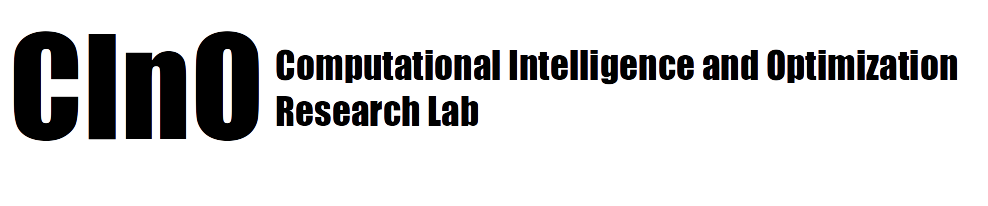
\includegraphics[scale = 0.2]{logos.png}
        \end{wrapfigure}
Inteligência Computacional é uma das áreas de Inteligência Artificial que lida com a aquisição de conhecimento automático. O nosso grupo está focado na teoria, aplicação e desenvolvimento de métodos de inteligência computacional .
	  
	  Optimização é uma das áreas de pesquisa operacional que lida com a encontrar as melhores soluções possíveis para os problemas . Nosso trabalho concentra-se na elaboração de teoria, modelos e algoritmos para problemas de optimização.


     \section{Programa de Pós-Graduação em Mecatrônica}  
O Programa de Pós-Graduação em Mecatrônica da UFBA (PPGM), programa de pós-graduação reconhecido pela CAPES, Engenharias III, é uma iniciativa conjunta da Escola Politécnica e do Instituto de Matemática (por meio do Departamento de Ciência da Computação) da Universidade Federal da Bahia. O PPGM visa prioritariamente formar docentes, pesquisadores e engenheiros com alto nível de qualificação em sistemas mecatrônicos, de forma a ser o PPGM o locus da integração Universidade-Empresa da região, no âmbito da Mecatrônica.
